\documentclass[10pt,a4paper]{article} 
\fontfamily{cmss}
\usepackage{amsmath}
\usepackage{amssymb}
\usepackage{mathtools}
\usepackage[brazilian]{babel}
\usepackage[utf8]{inputenc}
\usepackage[T1]{fontenc}
\usepackage[parfill]{parskip}
\usepackage[margin=1.0in]{geometry}
\usepackage{graphicx}
\usepackage{type1ec}
\usepackage{graphicx}
\usepackage{listings}

\begin{document}

	% CABECALHO %

	\begin{minipage}[b]{0.05\linewidth}
		%\begin{figure}
			
\includegraphics[scale=0.3]{ufmg}
		%\end{figure}
	\end{minipage}
	\hfill
	\begin{minipage}[b]{0.95\linewidth}
		\begin{flushright}
			\textbf{UNIVERSIDADE FEDERAL DE MINAS GERAIS} \\
			\textsc{Graduação em Engenharia de Sistemas} \\
			\textbf{Otimização Não Linear - Trabalho Computacional 1} \\
			2017-02 \\
			Prof. Felipe Campelo \\
			Matheus Silva Araujo - 2013066265
		\end{flushright}
	\end{minipage}

	\begin{center}
		\hrulefill
	\end{center}

	% CABECALHO %

	\section{Introdução}

	Métodos de direção de busca para otimização irrestrita partem da ideia básica de, a partir de um ponto, 
	encontrar um novo ponto na direção de decrescimento da função. E a partir desse novo ponto, repetir o processo
	até que um ponto que atenda os critérios desejados seja encontrado.

	A primeira implementação dessa ideia é o \emph{Método do Gradiente}, que encontra o novo ponto na reta definida pelo ponto corrente e
	o gradiente da função objetivo.

	Melhorias nessa implementação são feitas nos \emph{Métodos Quase-Newton}, que também consideram a curvatura da função.

	Quatro desses métodos serão avaliados nesse Trabalho Computacional.

	\section{Métodos analisados}

	Nesse Trabalho Computacional foram implementados quatro métodos usando \emph{Matlab}. Os quatro métodos foram avaliados usando duas funções objetivos.

	A seguir são apresentados os métodos e, posteriormente, os resultados obtidos.

	\subsection{Método do Gradiente}

	O \emph{Método do Gradiente} leva em consideração a avaliação do gradiente da função no ponto corrente.

	A ideia básica do método é encontrar o gradiente da função. Definida essa direção, um ponto de mínimo nessa direção é encontrado, 
	esse ponto passa a ser o novo ponto corrente e o método é repeito até que os critérios de parada sejam satisfeitos.

	Para utilizar esse método é necessário que a função objetivo seja diferenciável.

	Para o algoritmo implementado, o critério de parada utilizado foram as condições necessárias de primeira ordem, i.e., a norma do vetor gradiente deve se aproximar de 0.

	\subsection{Método de Newton Modificado}

	O \emph{Método de Newton} inclui na definição do novo ponto o cálculo da \emph{Hessiana} da função. Para funções quadráticas, a convergência acontecerá em apenas uma iteração. No entanto, para funções de maior ordem, o método usando puramente a \emph{Hessiana} pode não convergir.

	Para solucionar isso, é incluída uma pequena modificação no método, a minimização unidimensional em cada direção.

	Nesse método, é necessário que a função objetivo seja duas vezes diferenciável.

	O critério de parada utilizado na implementação do algoritmo foi o mesmo do método anterior.

	\subsection{Método da Família de Broyden}

	Os \emph{Métodos da Família de Broyden} incluem dois métodos: o \emph{Método BFP} e o \emph{Método BFGS}, nomeados em homenagem a seus autores. 

	Esses métodos constroem de forma iterativa uma matriz $\widetilde{H}_k$, equivalente à inversa da \emph{Hessiana} da função. A matriz $\widetilde{H}_k$ é então utilizada para definir o novo ponto.

	Os dois métodos se diferenciam apenas na fórmula usada para definir a matriz $\widetilde{H}_k$.

	Novamente, foi utilizada a redução da norma do gradiente como critério de parada na implementação do algoritmo.

	\subsection{Método do Gradiente Conjugado}

	O \emph{Método do Gradiente Conjugado} parte do sistema de equações lineares da forma:

	$$ Ax = b $$

	Define a minimalização da função:

	$$ f(x) = \frac{1}{2}x'Ax-bx+c $$

	E a partir dessa minimalização define $\beta_k$ que é utilizado na iteração.

	\section{Resultados}

	Para avaliar os algoritmos implementados foram utilizadas as duas funções $f_1$ e $f_2$, definidas a seguir:

	$$ f_1(x) = \sum_{i=1}^{n-1}100(x_{i+1}-x_i^2)^2+(1-x_i)^2 $$

	$$ f_2(x) = \sum_{i=1}^n \sum_{j=1}^{i} (x_j-j)^2 $$

	Para $f_1$ , $x_0 = [-1.2;1.0]$ e $f_2$, $x_0 = [5.0;5.0;...;5.0]$.

	\subsection{Função $f_1$}

	Para a função $f_1$, o único código implementado que convergiu para um ponto de mínimo foi o \emph{Método de Newton Modificado}. É possível que haja alguma falha na implementação dos algoritmos ou da própria função que não foi corrigida até o momento do envio do Trabalho.

	O \emph{Método de Newton} convergiu para o ponto $x = [0.838655; 0.707494]$, onde $f_1(x) = 0.0277572$, com 73 iterações e NCF\footnote{Número de chamadas de funções, quantidade de vezes em que a função objetivo foi avalida}=2012.

	O gráfico com as curvas da nível da função e os pontos da iteração é apresentado na Figura \ref{fig_f1_newton}.

	\begin{figure}[h]
		\centering
		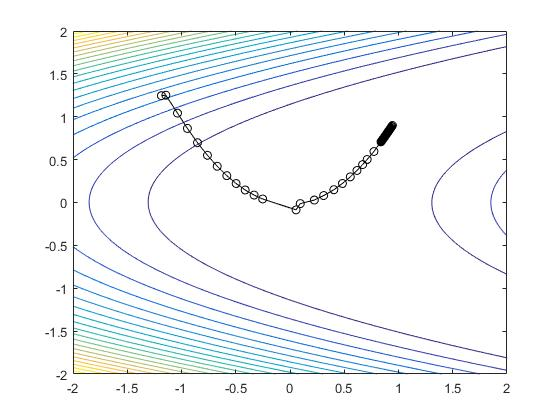
\includegraphics[width=11cm]{f1_newton}
		\caption{$f_1$ - \emph{Método de Newton Modificado}}
		\label{fig_f1_newton}
	\end{figure}

	\subsection{Função $f_2$}

	Já para a função $f_2$, os quatro métodos encontraram um ponto de mínimo. Os quatro métodos encontraram o mínimo próximo ao ponto $[1;2;3;4;5;6;7;8;9]$. De fato, $f_2 = 0$ nesse ponto.

	O método que convergiu mais rápido foi o \emph{Método de Newton}, com 12 iterações. No entanto, o que fez menor número de avaliações da função foi o \emph{Método do Gradiente Conjugado}, 821.

	Os resultados dos métodos são apresentados na Tabela \ref{tabela_f2}. Um gráfico do valor de $f_2(x)$ em função de NCF é apresentado na Figura \ref{fig_f2}.

	\begin{figure}[h]
		\centering
		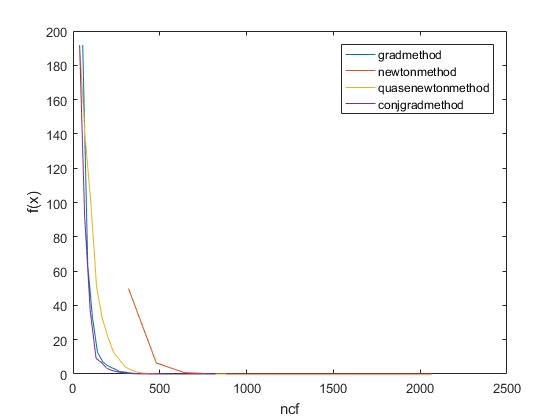
\includegraphics[width=11cm]{f2}
		\caption{$f_2(x)$ em função de NCF}
		\label{fig_f2}
	\end{figure}

\begin{table}[]
\centering
\caption{Resultados das avaliações para $f_2$}
\label{tabela_f2}
\begin{tabular}{|c|c|c|c|c|}
\hline
\textbf{Método}              & \textbf{Iterações} & \textbf{NCF}  & \textbf{Ponto}                                                                                                                                               & \begin{tabular}[c]{@{}c@{}}\textbf{Valor} \\ \textbf{no ponto}\end{tabular} \\ \hline
\emph{Gradiente}           & 31        & 1011 & \begin{tabular}[c]{@{}c@{}}1.000066\\ 2.000016\\ 3.000000\\ 4.000000\\ 5.000000\\ 6.000000\\ 7.000000\\ 8.000000\\ 9.000000\\ 9.995890\end{tabular} & 1.69374e-05                                               \\ \hline
\emph{Newton Modificado}   & 12        & 2065 & \begin{tabular}[c]{@{}c@{}}0.999951\\ 1.999838\\ 2.999725\\ 3.999613\\ 4.999500\\ 5.999387\\ 6.999275\\ 7.999162\\ 8.999049\\ 9.998937\end{tabular} & 1.24386e-05                                               \\ \hline
\emph{Família Broyden}     & 25        & 882  & \begin{tabular}[c]{@{}c@{}}0.999825\\ 1.999741\\ 2.999561\\ 3.999712\\ 4.999518\\ 5.999359\\ 6.999384\\ 7.999140\\ 8.999323\\ 9.999056\end{tabular} & 1.20232e-05                                               \\ \hline
\emph{Gradiente Conjugado} & 25        & 821  & \begin{tabular}[c]{@{}c@{}}0.999402\\ 1.999500\\ 2.999500\\ 3.999500\\ 4.999500\\ 5.999499\\ 6.999500\\ 7.999500\\ 8.999500\\ 9.995931\end{tabular} & 3.11331e-05                                               \\ \hline
\end{tabular}
\end{table}

	\section{Conclusão}

	Os quatro métodos foram implementados e apesar do insucesso na avaliação de $f_1$, em $f_2$ os quatro métodos encontraram o mínimo próximo ao mesmo ponto.

	Para $f_2$, os quatro métodos encontraram suficientemente próximos do ponto de mínimo.

	O \emph{Método de Newton Modificado} precisou de um número menor de iterações, no entanto, fez o maior número de avaliações da função, para calcular a Hessiana.

	Já os métodos do \emph{Gradiente Conjugado} e da \emph{Família Broyden} fizeram um número pouco menor de iterações do que o \emph{Método do Gradiente} e precisam de menos avalidações da função.

\end{document}
